\subsection{Pooling Layers}
\begin{frame}{}
    \LARGE CNN Layer: \textbf{Pooling Layers}
\end{frame}

\begin{frame}[allowframebreaks]{Pooling}

\begin{itemize}
    \item Compute mean or max over small windows to reduce resolution
\end{itemize}


\begin{figure}
\centering
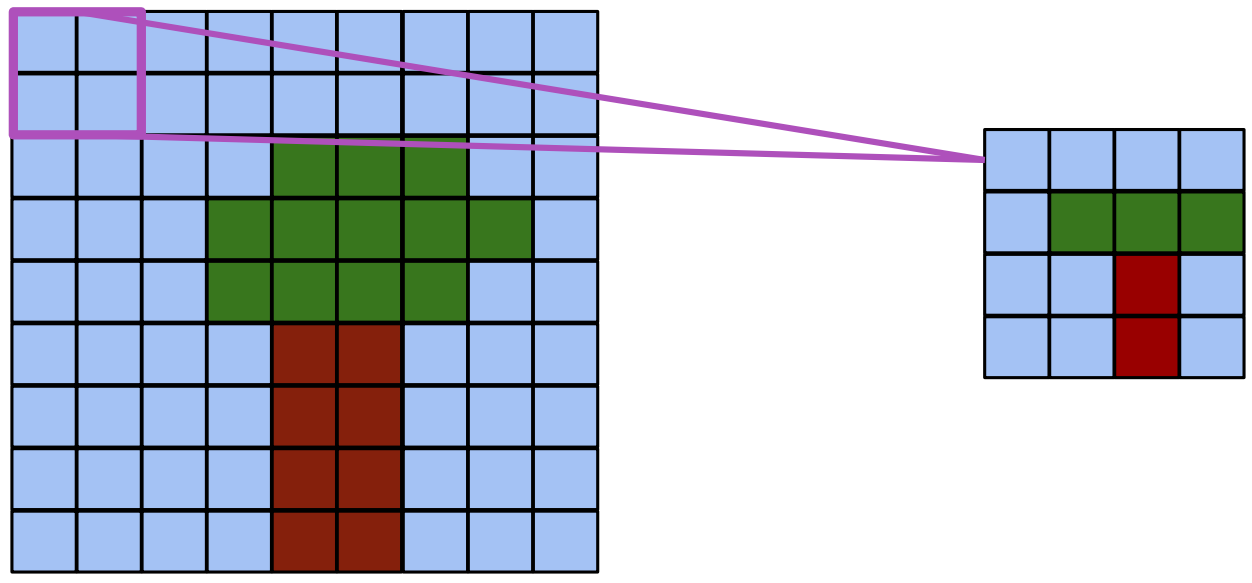
\includegraphics[width=1.0\textwidth,height=0.8\textheight,keepaspectratio]{images/cnn/pool_1.png}
\end{figure}

\framebreak

\begin{figure}
\centering
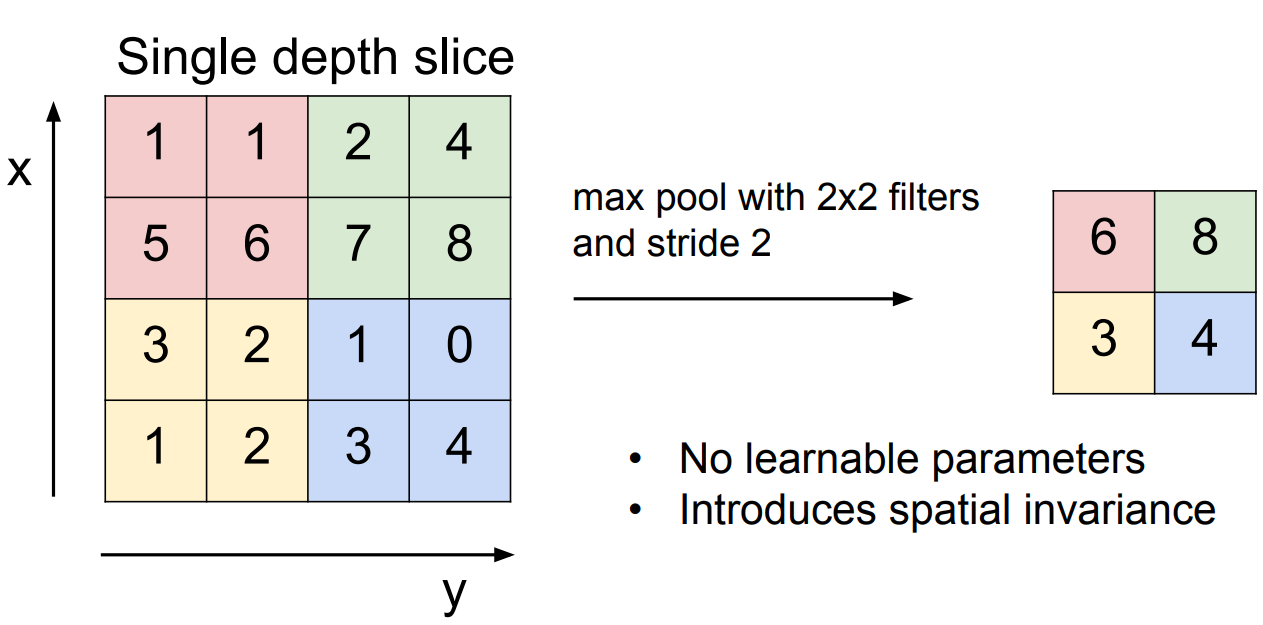
\includegraphics[width=1.0\textwidth,height=0.8\textheight,keepaspectratio]{images/cnn/pool_2.png}
\end{figure}
    
\end{frame}

\begin{frame}[fragile]{Pooling Layers}
\begin{block}{Purpose:}
    \begin{itemize}
        \item Downsample feature maps, reduce spatial dims and parameters, add invariance.
    \end{itemize}
\end{block}

\begin{block}{Types:}
    \begin{itemize}
        \item Max Pooling
        \item Average Pooling
        \item Global Average Pooling
        \item Global Max Pooling
    \end{itemize}
\end{block}

\begin{lstlisting}[language=Python, caption={Code snippet (PyTorch)}, basicstyle=\ttfamily\footnotesize]
import torch.nn as nn

pool = nn.MaxPool2d(kernel_size=2, stride=2)
pooled = pool(x)  # halves H and W
\end{lstlisting}
\end{frame}  

\begin{frame}[allowframebreaks]{Pooling Layers}
    \begin{figure}
    \centering
    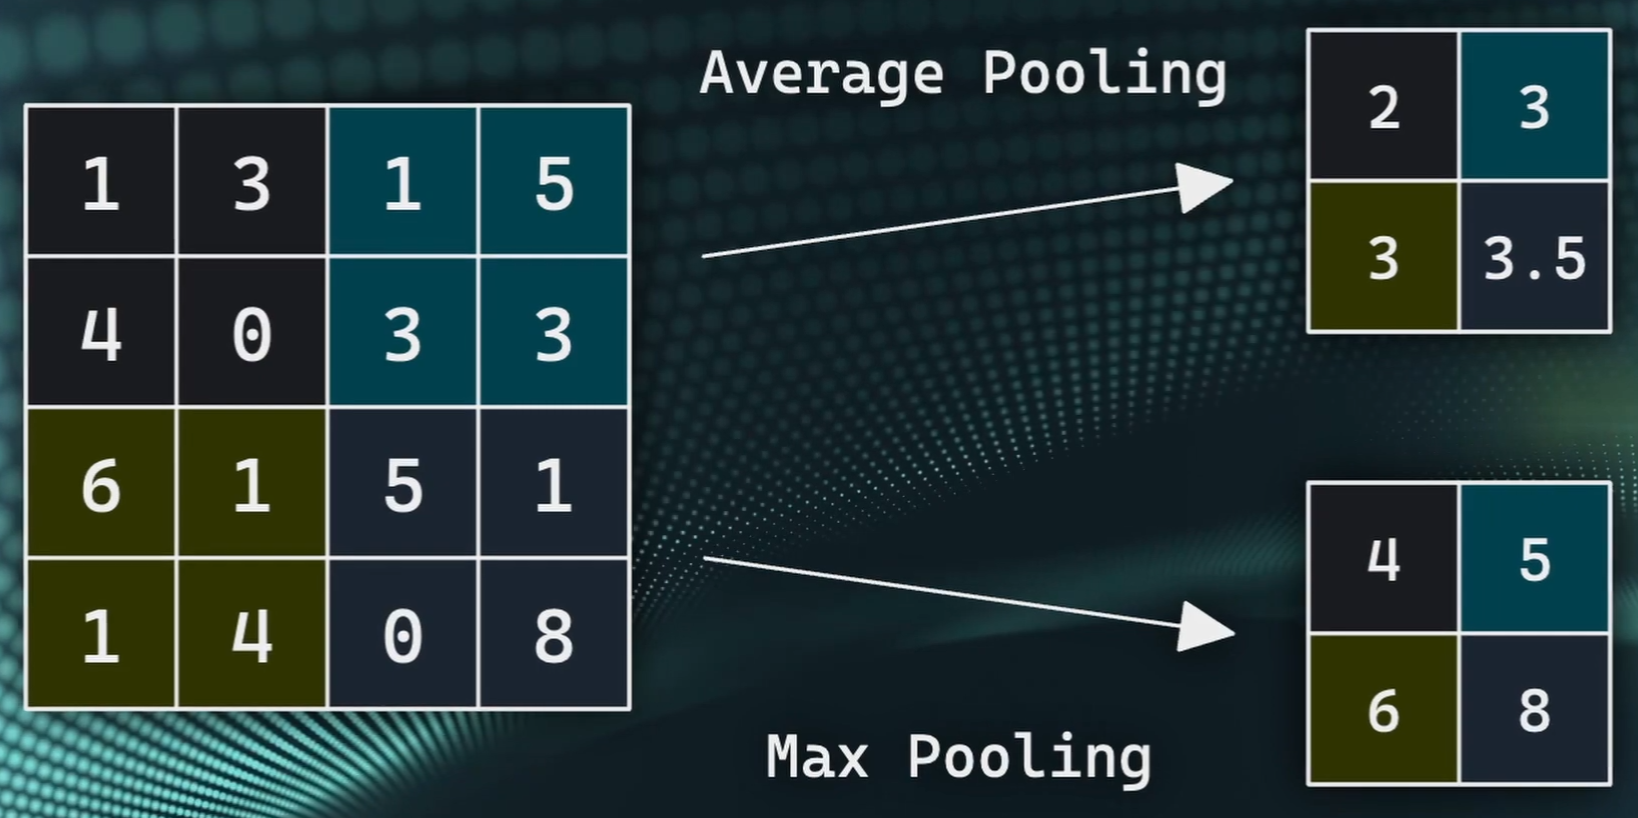
\includegraphics[width=0.95\textwidth,height=0.95\textheight,keepaspectratio]{images/cnn/pooling-layer.png}
    \end{figure}
\end{frame}

\begin{frame}[allowframebreaks]{Convolutions on RGB images}
    \begin{figure}
    \centering
    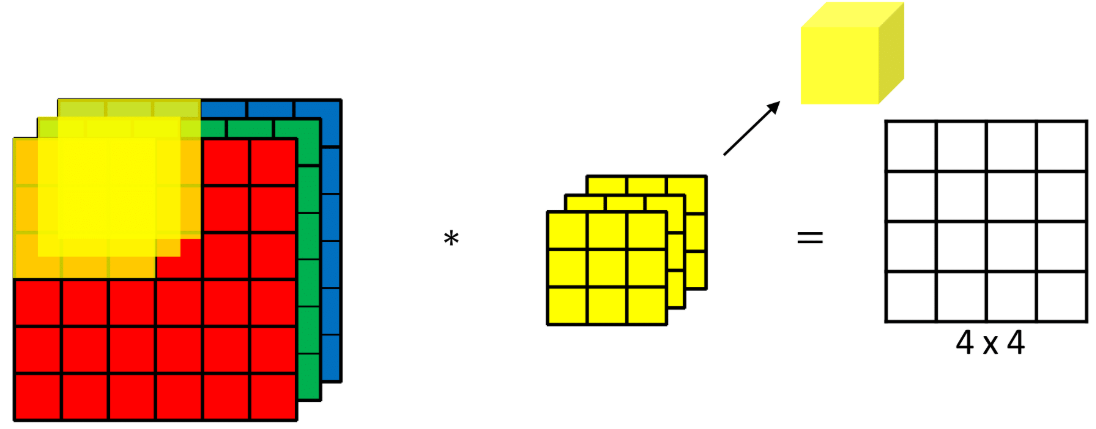
\includegraphics[width=0.95\textwidth,height=0.95\textheight,keepaspectratio]{images/cnn/rgb-convolution.png}
    \end{figure}
\end{frame}

\begin{frame}[allowframebreaks]{Multiple Channels \& Multiple Filters}
    \begin{figure}
    \centering
    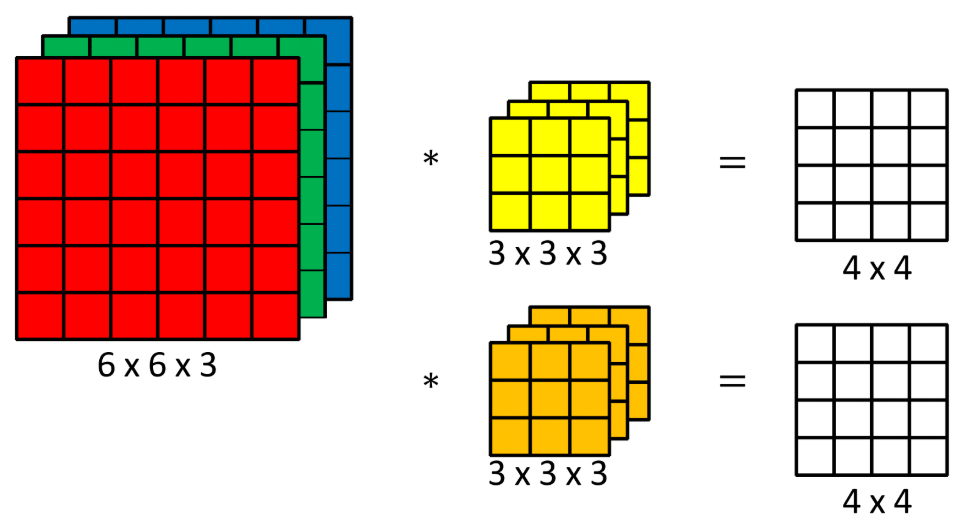
\includegraphics[width=0.95\textwidth,height=0.95\textheight,keepaspectratio]{images/cnn/mutiple-filters.png}
    \end{figure}
\end{frame}

\begin{frame}[allowframebreaks]{Number of Parameters?}
    \LARGE If you have 10 filters of size $3 \times 3 \times 3$ in one layer of a neural network, how many parameters does that layer have?

\framebreak
    Each filter has size $3 \times 3 \times 3 = 27$ parameters (weights).  \\[2em]
    With 10 filters: $10 \times 27 = 270$ weights.  \\[2em]
    If each filter also has a bias term, add 10 more parameters: \textbf{$270 + 10 = 280$} parameters in total.
\end{frame}